% 
\documentclass[a4paper,10pt]{article}
\usepackage[utf8x]{inputenc}
\usepackage[OT1]{fontenc}
\usepackage{hyperref}
\usepackage{Sweave}
\usepackage{graphicx}
\usepackage{color}
\graphicspath{{figures/}}
%\usepackage{float}
\usepackage{wrapfig}
%\usepackage{subfigure}
%% Package to linebreak URLs in a sane manner.
\usepackage{url}
%% Define a new 'smallurl' style for the package that will use a smaller font.
\makeatletter
\def\url@smallurlstyle{%
  \@ifundefined{selectfont}{\def\UrlFont{\sf}}{\def\UrlFont{\small\ttfamily}}}
\makeatother
%% Now actually use the newly defined style.
\urlstyle{smallurl}
%% Define 'tinyurl' style for even smaller URLs (such as in tables)
\makeatletter
\def\url@tinyurlstyle{%
  \@ifundefined{selectfont}{\def\UrlFont{\sf}}{\def\UrlFont{\scriptsize\ttfamily}}}
\makeatother
%% Make margins less ridiculous
\usepackage{fullpage}
%% Make URLs clickable
%\usepackage[colorlinks, bookmarks=false]{hyperref}
%\usepackage[colorlinks, bookmarks=true]{hyperref}
%% Since I'm using the LaTeX Makefile that uses dvips, I need this
%% package to make URLs break nicely
\usepackage{breakurl}
\usepackage{todonotes}
\usepackage{amsmath,amsfonts}
\numberwithin{equation}{subsection}
%%\usepackage{nonfloat}
\usepackage{bbm}
\usepackage{setspace}
\onehalfspacing
\usepackage{tabularx}

%
%
%
\usepackage{listings}
\usepackage{courier}
\lstset{
         basicstyle=\footnotesize\ttfamily, % Standardschrift
         %numbers=left,               % Ort der Zeilennummern
         numberstyle=\tiny,          % Stil der Zeilennummern
         stepnumber=2,               % Abstand zwischen den Zeilennummern
         numbersep=5pt,              % Abstand der Nummern zum Text
         tabsize=2,                  % Groesse von Tabs
         extendedchars=true,         %
         breaklines=true,            % Zeilen werden Umgebrochen
         keywordstyle=\color{red},
    		frame=b,         
 %        keywordstyle=[1]\textbf,    % Stil der Keywords
 %        keywordstyle=[2]\textbf,    %
 %        keywordstyle=[3]\textbf,    %
 %        keywordstyle=[4]\textbf,   \sqrt{\sqrt{}} %
         stringstyle=\color{white}\ttfamily, % Farbe der String
         showspaces=false,           % Leerzeichen anzeigen ?
         showtabs=false,             % Tabs anzeigen ?
         xleftmargin=17pt,
         framexleftmargin=18pt,
         framexrightmargin=6pt,
         framexbottommargin=4pt,
         %backgroundcolor=\color{lightgray},
         showstringspaces=false      % Leerzeichen in Strings anzeigen ?        
 }
 \lstloadlanguages{% Check Dokumentation for further languages ...
         %[Visual]Basic
         %Pascal
         %C
         %C++
         %XML
         %HTML
         Java
 }
%\DeclareCaptionFont{blue}{\color{blue}} 
%\captionsetup[lstlisting]{singlelinecheck=false, labelfont={blue}, textfont={blue}}
\usepackage{caption}
\DeclareCaptionFont{white}{\color{white}}
\DeclareCaptionFormat{listing}{\colorbox[cmyk]{0.43, 0.35, 0.35,0.01}{\parbox{\textwidth}{\hspace{15pt}#1#2#3}}}
\captionsetup[lstlisting]{format=listing,labelfont=white,textfont=white, singlelinecheck=false, margin=0pt, font={bf,footnotesize}}
%
%

\begin{document}

\title{Mining of Android SCM}
\author{Pavel Senin}

\maketitle

\begin{abstract}
Both, software product improvement and software process improvement, require in-depth understanding 
of current project state. Here I present an approach for exploration of a software repository by 
using Software Trajectory code. I will explore Android SCM system\ldots
\end{abstract}

\section{Introduction}
According to the Android home website, \url{http://source.android.com/}: ``Android is an 
open-source software stack for mobile phones and other devices''.

Initial developer of the software, Android Inc. - a small startup company - was purchased by Google 
in in 2005. In November 2007 the Open Handset Alliance, a consortium of 84 companies, announced 
availability of the Android Software Development Kit (SDK). The open Open Handset Alliance was formed 
of hardware, software, and telecommunication companies (including Intel, HTC, ARM, Samsung and Motorola)
and devoted to advancing of open standards for mobile devices. 

\begin{wrapfigure}{l}{0.5\textwidth}
   \begin{center}
   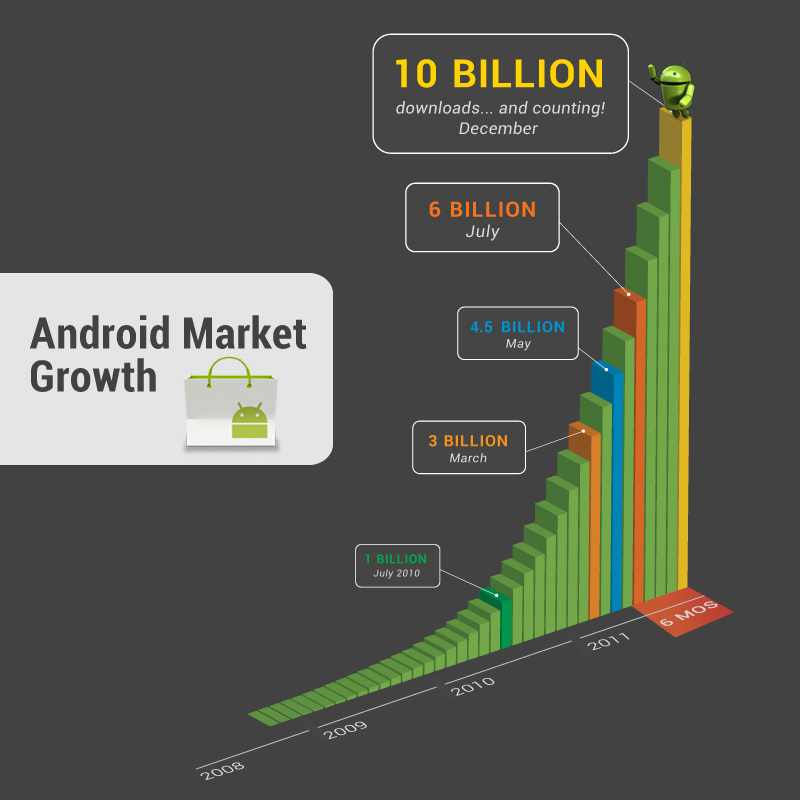
\includegraphics[scale=0.3,width=0.48\textwidth]{graph_only_3}
   \end{center}
   \caption{The Android store downloads timeline.}
   \label{fig:android_downloads}
\end{wrapfigure}

The Android code is open-source and released under the Apache License; it is a complete 
mobile platform built on the monolithic Linux 2.6 kernel. The Android platform provides 
developers with an SDK which consist of a set of development tools, debugger and a true emulator. 
There are an Eclipse plugin, a set of libraries a multimedia user interface, and a core set of 
phone applications. The Android application model alleviates the cost of software development by 
allowing extending, replacing, and reusing of existing software components. The Dalvik virtual 
machine, which is the part of Android distribution, provides a way to maximize application portability, 
performance and security. Android OS allows true application multitasking, provides rich user 
notifications and customizable home screens with resizable widgets. Latest, 4.0 version of
Android System provides streaming voice recognition.

Currently, the Android Open Source Project (AOSP) is led by Google and includes not only the 
original members of OHA but many other companies. The role of AOSP is to maintain and develop 
Android.

Including Beta, there were 10 major releases of Android as well as a number of intermediate 
releases. All releases prior to 2.0 were for mobile phones exclusively. Since 2.0 release 
Android OS is a tablet-oriented operating system. Most of the mobile devices at market use 
2.x version of Android. The 3.0 release, Honeycomb, does not officially run on phones; 
the latest 4.0 release, Ice Cream Sandwich, runs on all mobile devices.

In Q3, 2011 (November 15, 2011) Android officially become the most popular OS for newly sold mobile 
devices. In December 2011 there were registered 10 billions of downloads from Android store called
Android Marketplace. 

\section{MSR 2012 Challenge}
The research field of Mining Software Repositories (MSR) is focused on analyzes of the rich 
data available in software repositories. The immediate goal of such research is to infer interesting 
and actionable information about software systems and projects. While there are multiple scientific 
events where researchers working in the field meet, the Mining Software Repositories 
conference considered to be the major meeting event. The 2012 MSR conference is a 9th such event
and is collocated with ICSE -the International Conference on Software Engineering.
Along with the research track since 2006 the MSR conference includes the Mining Challenge where 
researchers demonstrate application of their tools to the selected repository mining problem. This
year Android platform was selected for the challenge. Two XML files containing change and bug report 
data were offered to participants to uncover interesting facts related to the Android platform.

\lstset{label=changeXSDFragment,caption=List of metadata provided by change trail XML (fragment) }
\begin{lstlisting}
 <xs:element name="change">
    <xs:complexType>
      <xs:sequence>
        <xs:element ref="project"/>
        <xs:element ref="commit_hash"/>
        <xs:element ref="tree_hash"/>
        <xs:element ref="parent_hashes"/>
        <xs:element ref="author_name"/>
        <xs:element ref="author_e-mail"/>
        <xs:element ref="author_date"/>
        <xs:element ref="commiter_name"/>
        <xs:element ref="commiter_email"/>
        <xs:element ref="committer_date"/>
        <xs:element ref="subject"/>
        <xs:element ref="message"/>
        <xs:element ref="target"/>
      </xs:sequence>
    </xs:complexType>
  </xs:element>
\end{lstlisting}

\section{Data.}
Two XML files were offered for the MSR challenge. These files contain the most of the information
obtainable from Google-hosted source code repository (Git) as well as Google-hosted bug and issue
tracking system (Google project hosting). 
The full XSD for both XML files can be found in the Appendix section of this report.
While the issues and comments trail \ref{bugsXSD} provided nearly complete information,
the change trail \ref{changeXSD} provided for a challenge contained only the high-level change information.
The thirteen data fields of the change trail XSD file shown at the fragment Listing \ref{changeXSDFragment}. 
The provided data contains information about revision tree, author and a commiter identification, change
message and affected targets.
Since I am focusing on mining of temporal patterns for inferring recurrent behaviors, I consider 
this provided dataset rather poor since it lacks many of auxiliary change and target information. 
In fact, among relevant to Trajectory toolkit data fields, every timestamped entity of the offered trail
containe only author id and an indication of affected targets (the committer information
is rather useless for trajectory since it could not be trusted due to the nature of git merged commits).   

\begin{wrapfigure}{l}{0.5\textwidth}
   \begin{center}
   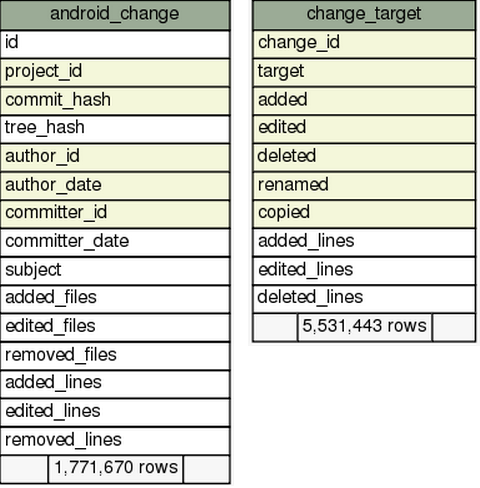
\includegraphics[scale=0.4,width=0.5\textwidth]{schema-change-fragment}
   \end{center}
   \caption{The Trajectory DB schema fragment. Change and target tables shown.}
   \label{fig:android_downloads}
\end{wrapfigure}

\subsection{Auxiliary information collection and data organisation.}
In order to enrich the provided data for recurrent pattern analysis I decided to enrich offered by MSR
challenge dataset with auxiliary information. I used existing change information (commit hash) to 
query Android repository for retrieval of data indicating whether the affected within a commit target 
was added, modified or deleted along with quantitative summary about that target change - the amount of 
lines added, modified or deleted. I have coded the auxiliary information retrieval module using Java and
JGit API, this module extends existing Trajectory SCM connectors.

Trajectory is using database backend for all the analysis need. The existing database schema was altered
to logically incorporate structure of Android SCM data. The main tables of the database correspond to
entities of change log and issue log. There are separate tables for change targets and issue comments.
Schema is further organized around these tables, normalized and indexed in order to speed up search.

Some additional information concerned the retrival of data need to be added here.

\section{Threats to Validity}
Before discussing the mining methodology and findings I discuss several threats to validity and how 
I have addressed them. These includeg general threats to construct validity, external validity,
and specific threats to my particular methodology, including repository threats, recall and 
precision threats.

\subsection{General threats.}
Construct validity requires that Trajectory must correctly identify authors and corresponding activity
along with quantitative data. First of all, it is hard to access how much of the contributor's activity 
is actually captured within the trails provided for MSR Challenge and in Android OS SCM. I just assume 
that provided and retrieved data represent a valid trail of commits into SCM and will and will not 
claim external validity and draw any general conclusions about all or part of Android software. 

\subsection{Repository data threats.}
The information enclosed for the challenge appears to be not reproducible due to the changes happened 
within the Android OS hosting scheme. Based on my own retrieval of the auxiliary data, it is impossible 
to confirm about 40\% of the commits for various reasons. 
(I can actually put categories and numbers here, something like
1771670 rec in XML from which 714025 are nulls)\ldots 
\ldots analogous to previous research, I can determine sort of ``confusion matrix'' by 
randomly sampling 200 null commits from each project and manually verifying whether or not they 
are indeed nulls or Trajectory pipeline failed \ldots. 
All of my data is retrieved from Git repositories. Git is known to track records of each 
developer’s local time and the time zone with a commit. Thus the potential imprecisions
in time-of-day results are negligible. I believe that all of the developers are have accurate local 
time on their workstations.
I ignore Git merge commits as well as cherry-pick commits which tend to only record metadata about 
integration between different maintainers’ trees.

\subsection{Threats to commit characteristics.}
Despite the nature of Android community development model where commits may be performed by 
Android OS maintainers who merge data from external contributors, Git preserves commit metadata 
from original authors. I use the author\_date field in my analyses for the change time-stamp identification 
thus avoiding any confusion.
There is a treat to changes which belong to contributors with several email addresses. \ldots, must be addressed.

\section{Data curation.}
In order to proceed with patterns mining apply Trajectory framework After the collection of auxiliary data The data collected at the previous step was filtered into the separate database table for further analyses.
The reason to perform this step was the overall amount of merged commits as well as the amount of commits
which lacked the auxiliary data.

\section{Android SCM facts}
There are 1771667 changes registered in the repository. First change commit to Android repository dates back 
to Monday January 12th 1970, 14:46:40 and belongs to Upstream, while the last change
within the analyzed data set belongs to to Guy Zadickario and dated 
Tuesday June 21st 2011, 12:41:41.

As per January, 1, 2012 Android repository contains a total of 26851267 lines of source code in 
152225 files. 

\begin{table}
  \caption{Android repository snapshot source code metrics.}
  \begin{tabularx}{\textwidth}{ | X | r | r | r | r | r |}
  \hline                       
  Nb. files & Language & Total lines & Source & Blanks & Comments \\
  \hline 
  Assembly &3391 & 565314 & 426104 & 60673 & 98215 \\
  IDL & 78 & 7926 & 7174 & 752 & 640 \\
 Perl & 348 & 105024 & 75877 & 13999 & 18975 \\    
  CSS & 224 & 38417 & 30687 & 5899 & 2033 \\
  XML & 10090 & 5963665 & 5762297 & 59093 & 143243 \\   
  Matlab & 889 & 62911 & 51323 & 10715 & 3911 \\
  Text & 7563 & 1669710 & 0 & 93271 & 1576439 \\
  FlashParameter & 3 & 364 & 265 & 40 & 59 \\
  C & 42151 & 9979284 & 6676807 & 1278259 & 2363003 \\   
  shell & 3930 & 2476537 & 1986936 & 207861 & 288125 \\  
  JavaScript & 5347 & 866236 & 511330 & 131581 & 225745 \\   
  Java & 251129 & 5265723 & 3152054 & 639535 & 1509917 \\
  HTML & 6209 & 1208415 & 1062506 & 100306 & 61760 \\
  make & 3506 & 512065 & 377850 & 62696 & 71518 \\
  Awk & 21 & 2762 & 1778 & 226 & 871 \\
  SQL & 3 & 454 & 454 & 0 & 0 \\
  Pascal & 160 & 15681 & 2555 & 372 & 13334 \\      
  Python & 912 & 190278 & 132202 & 30889 & 27888 \\ 
  PHP & 180 & 50137 & 39060 & 2268 & 9218 \\
  C++ & 31390 & 9228878 & 6262708 & 1318921 & 1835150 \\   
  Jess & 2 & 246 & 192 & 54 & 0 \\
  CSharp & 66 & 6513 & 5282 & 643 & 596 \\      
  Lisp & 10633 & 493777 & 285826 & 86471 & 176378 \\
  \hline     
  TOTAL & 152225 & 38710317 & 4104524 & 8427018 & 26851267 \\    
  \hline  
  \end{tabularx}
\end{table}

\section{Data reduction and indexing}

\section{Results}


\section{Future work}
Ultimately by application of Trajectory I want to discover recurrent behaviors from
software process artifacts trails. This data can be further applied to improve the
productivity of development.


\clearpage
\lstinputlisting[label=bugsXSD,caption=Bugs XML file schema]{bugs.xsd}

\clearpage
\lstinputlisting[label=changeXSD,caption=Change XML file schema]{git.xsd}

\bibliographystyle{abbrv}
\bibliography{seninp}

\end{document}
